% The annotation project cycle — diagram for docs/annotation-cycle.md
% Build:  pdflatex annotation-cycle.tex
%         pdftocairo -svg annotation-cycle.pdf annotation-cycle.svg
\documentclass[border=8pt]{standalone}
\usepackage{tikz}
\usepackage[scaled]{helvet}
\renewcommand\familydefault{\sfdefault}
\usetikzlibrary{arrows.meta, calc, backgrounds}

\definecolor{cDefine}{HTML}{D7E3FC}  % define  — blue
\definecolor{cDefineL}{HTML}{3B6FD4}
\definecolor{cDist}{HTML}{D5ECDD}    % distribute — green
\definecolor{cDistL}{HTML}{2E8B57}
\definecolor{cAssess}{HTML}{FBE0DC}  % assess/evolve — warm
\definecolor{cAssessL}{HTML}{C0522D}
\definecolor{ink}{HTML}{1F2933}
\definecolor{muted}{HTML}{6B7280}

\begin{document}
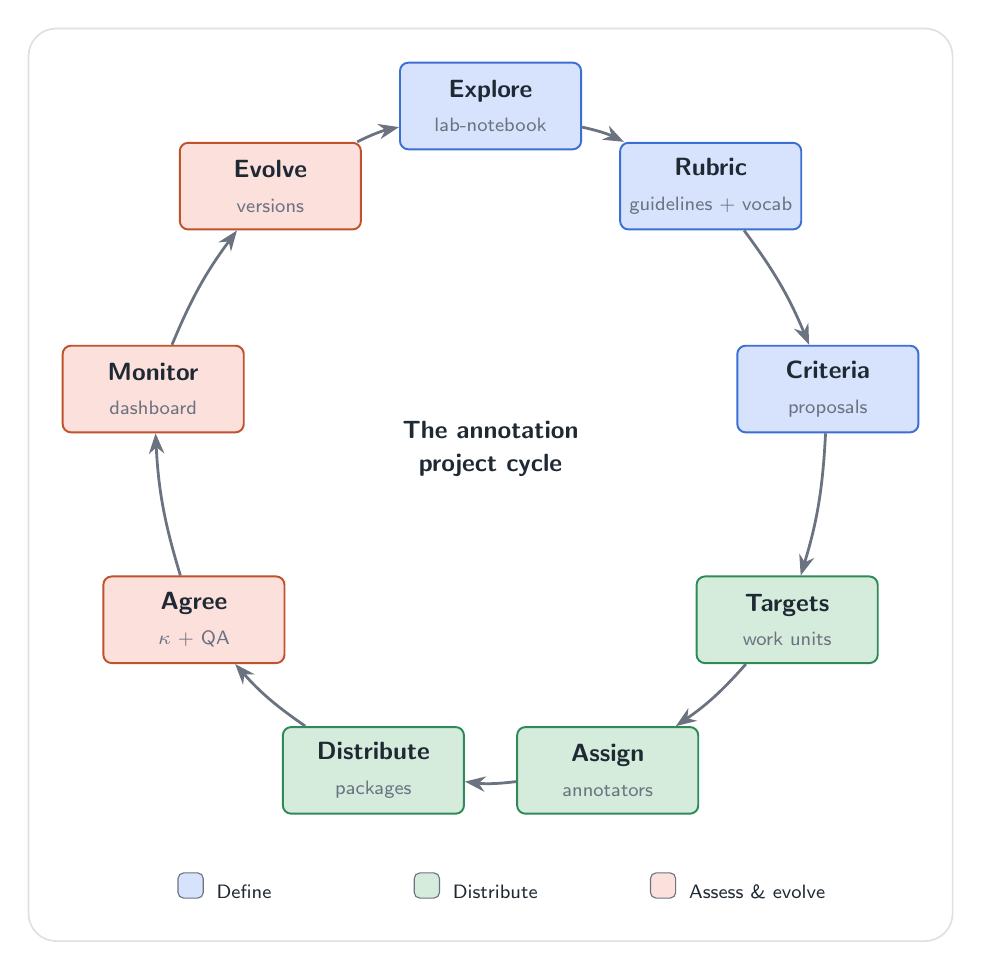
\begin{tikzpicture}[
  % Self-contained light panel so the figure stays legible on any page theme
  % (incl. dark mode), where a transparent background would be dark-on-dark.
  show background rectangle,
  inner frame sep=12pt,
  background rectangle/.style={fill=white, draw=black!12, line width=0.6pt,
                               rounded corners=10pt},
  >={Stealth[length=2.6mm]},
  font=\small,
  stage/.style={
    rounded corners=3pt, draw, line width=0.7pt,
    minimum width=23mm, minimum height=11mm, align=center,
    inner sep=2pt, text=ink, fill=#1,
  },
  arr/.style={->, line width=1.0pt, color=muted},
]
  \def\R{4.35cm}

  % --- nodes on a ring, clockwise from the top ---
  \foreach \i/\ang/\name/\sub/\fill/\edge in {
      1/ 90/Explore/{lab-notebook}/cDefine/cDefineL,
      2/ 50/Rubric/{guidelines + vocab}/cDefine/cDefineL,
      3/ 10/Criteria/{proposals}/cDefine/cDefineL,
      4/330/Targets/{work units}/cDist/cDistL,
      5/290/Assign/{annotators}/cDist/cDistL,
      6/250/Distribute/{packages}/cDist/cDistL,
      7/210/Agree/{$\kappa$ + QA}/cAssess/cAssessL,
      8/170/Monitor/{dashboard}/cAssess/cAssessL,
      9/130/Evolve/{versions}/cAssess/cAssessL%
  }{
    \node[stage=\fill, draw=\edge] (n\i) at (\ang:\R)
      {\textbf{\name}\\[1.5pt]{\scriptsize\textcolor{muted}{\sub}}};
  }

  % --- clockwise arrows closing the ring ---
  \foreach \i/\j in {1/2,2/3,3/4,4/5,5/6,6/7,7/8,8/9,9/1}{
    \draw[arr] (n\i) to[bend left=7] (n\j);
  }

  % --- centre label ---
  \node[align=center, text=ink] at (0,0)
    {\textbf{The annotation}\\[1pt]\textbf{project cycle}};

  % --- phase legend ---
  \begin{scope}[shift={(0,-5.55cm)}]
    \foreach \k/\lab/\c in {0/Define/cDefine, 1/Distribute/cDist, 2/{Assess \& evolve}/cAssess}{
      \node[anchor=west] at ({-4.1cm + \k*3.0cm}, 0)
        {\tikz\node[rounded corners=2pt, draw=muted, line width=0.4pt,
                    minimum width=3.2mm, minimum height=3.2mm, fill=\c]{};\,
         {\scriptsize\textcolor{ink}{\lab}}};
    }
  \end{scope}
\end{tikzpicture}
\end{document}
